\documentclass{article}
\usepackage{graphicx}
\usepackage{amsmath} % For math formatting


\begin{document}

\title{Fall-2023 5304 LecN1 Notes}
\author{Wan}
\date{\today}
\maketitle

\noindent
Topics: Introduction; Types of problems seen in this course; Math background;
Matrices; Eigenvalues and Eigencevectors; Null space and range; Rank; Types of matrices;
Special Matrices.

\section{Matrix Multiplication}

\subsection*{Matrix-Matrix Multiplication}


\subsection*{Matrix-Vector Multiplication, 2 Ways}
\textbf{Form 1: Dot product view}\\
\\
\textbf{Form 2: Linear combination view}
In this view, vector can be treated as a place storing the coefficients
of the column of matrix A.


\subsection*{Vector-Matrix Multiplication, 2 Ways}

\subsection*{Vector-Vector Multiplication, 2 Ways}
\textbf{Form 1: Inner product view}
This is a scalar.
\\
\textbf{Form 2: Outer product view}
Will produce rank-1 matrix.

\subsection*{A x B = C, get jth col of C}
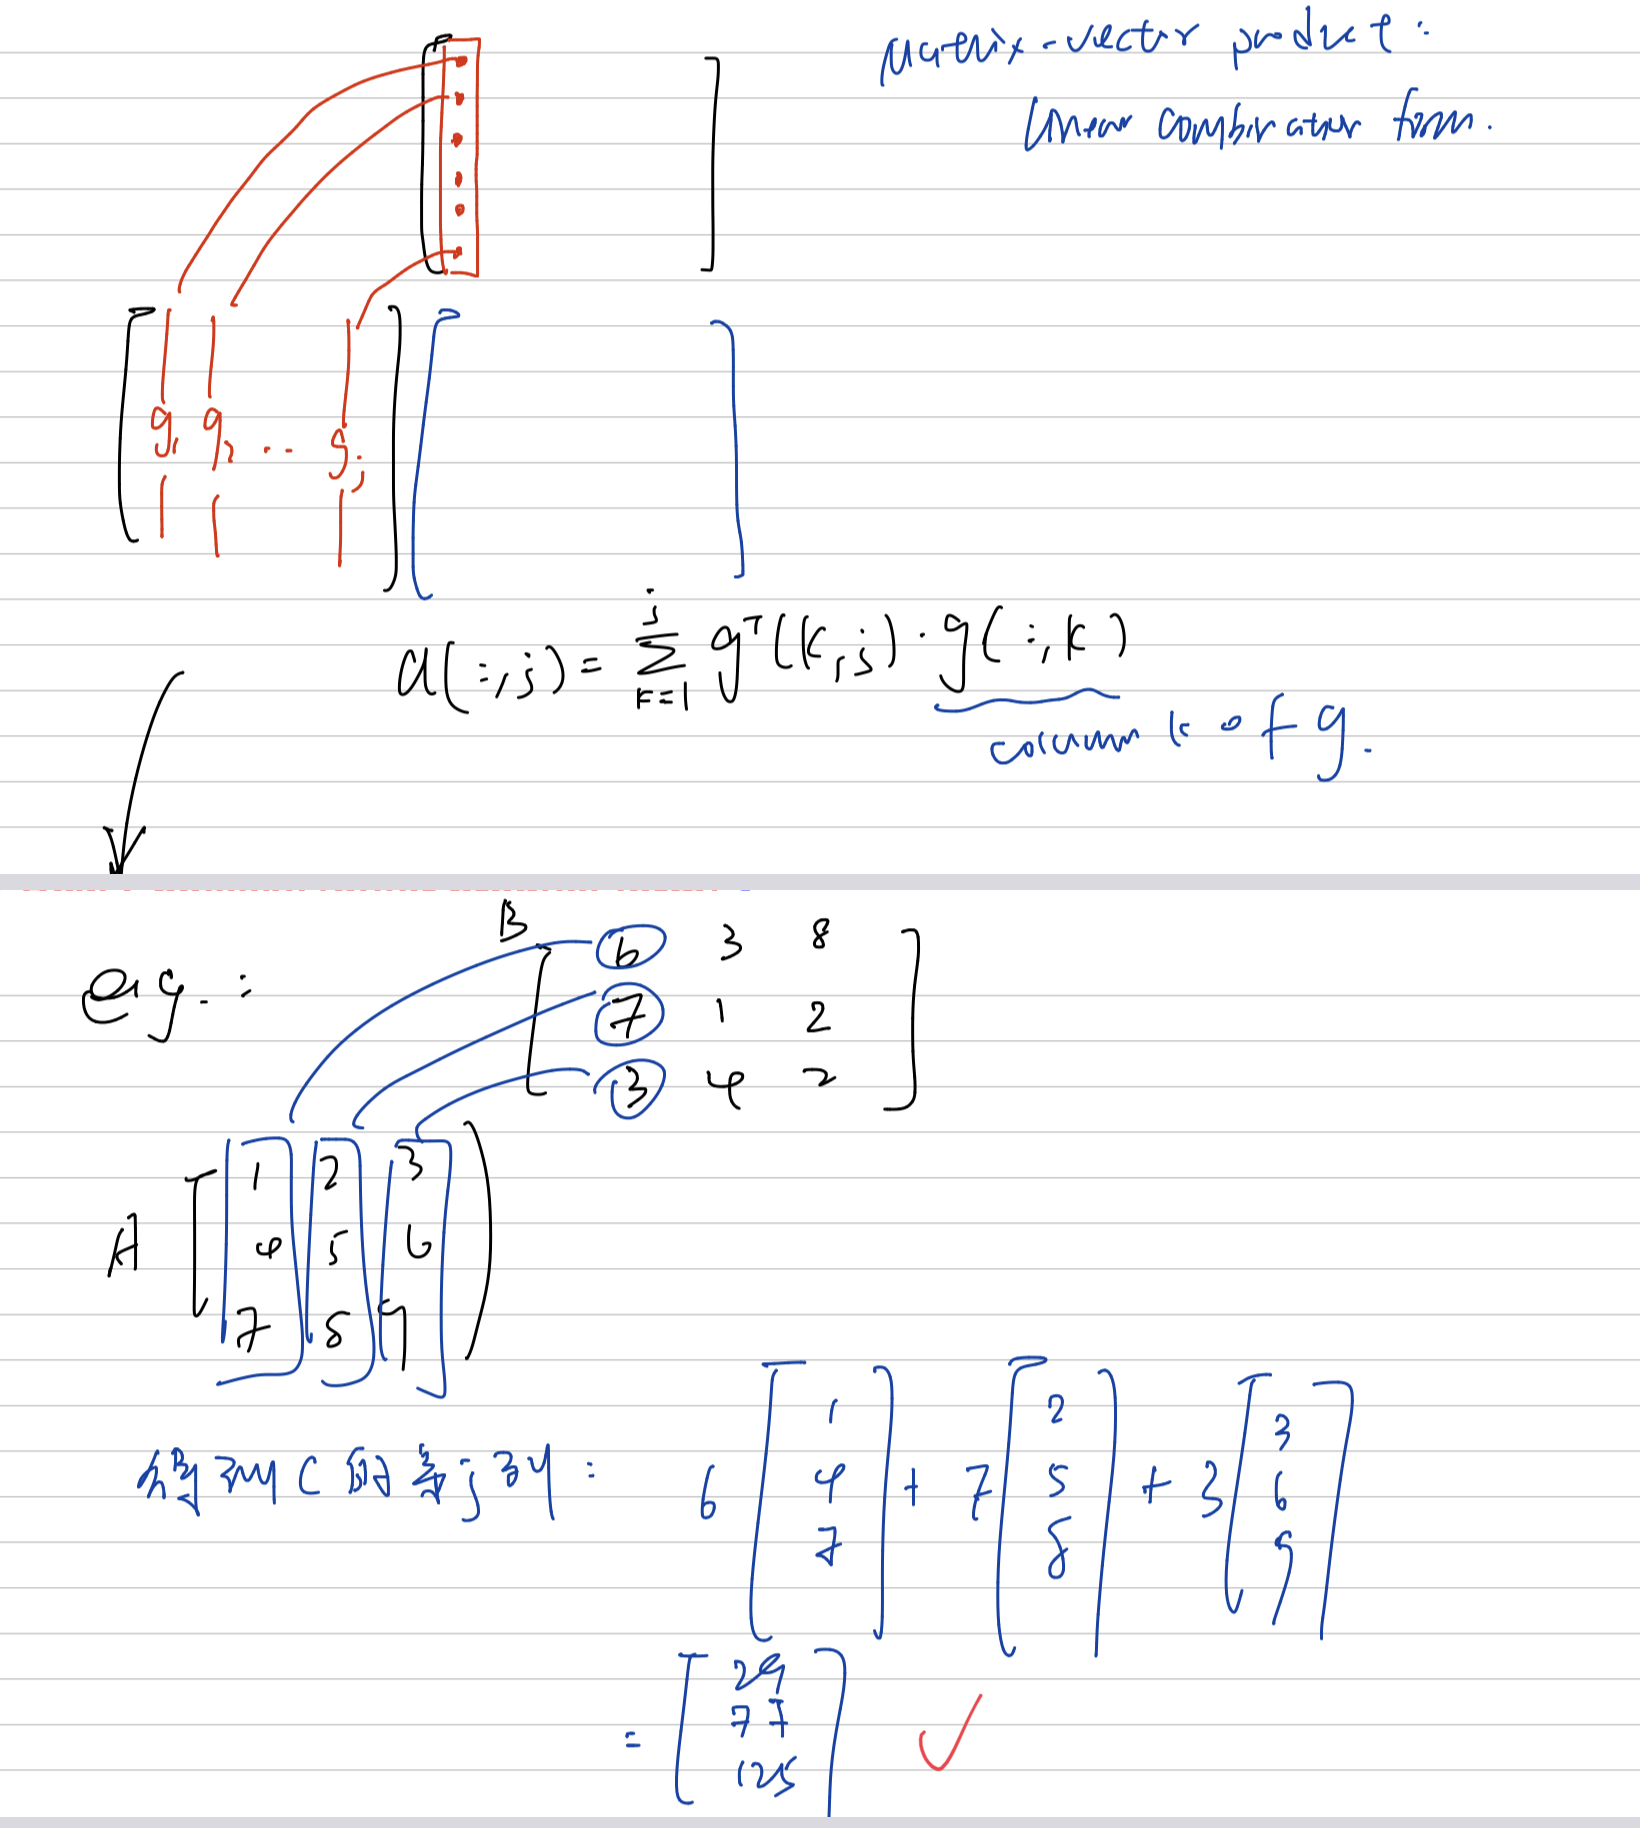
\includegraphics[width=1\linewidth]{1-1}


\pagebreak
\section{Rank}

\subsection*{Rank + Nullity Theorem}

\subsection*{Some Conclusions/Facts}
1, A full rank matrix X, and a nonzero vector v, $Xv \neq 0$\\
2, If A is a nonsingular, square matrix, full rank, then $A^{-1}$ is full rank. $R(A) = R(A^{-1})=n$\\
3, If we have a matrix A and a full rank matrix Q, then R(A) = R(QA) = R(AQ). i.e., useing Q left-multiply a matrix
or right-multiply a matrix will not change the rank of the original matrix.\\



\section{Special Matrices}
\subsection*{Diaguonal Matrix}
\subsection*{Vandermond}
\subsection*{Hermitan}
Def: $A^H = A$



\subsection*{Unitary}
Def: $Q^TQ = QQ^T = I$, or $Q^{-1} = Q^T$

\subsection*{Orthogonal}
Def: $Q^TQ = I$ [orthonormal columns] \\
% 正交归一
A matrix is orthogonal iff its columns are orthonormal, meaning they are orthogonal and of unit length.\\
A set of vectors is said to be orthonormal if they are all normal, and each pair of vectors in the set is orthogonal. \\
\includegraphics[width=1\linewidth]{1-3}

\medskip
\noindent
Properties:\\
det(Q) = ± 1. 

\medskip
\noindent
Geometric understanding:\\
Rotation matrices are orthogonal.

\medskip
\noindent
Application:\\
- decompositions in numerical linear algebra: QR, SVD.
- Orthogonality is essential in understanding and solving least-squares problems.

\medskip
\noindent
Note: \\
- its difference with unitary (orthogonal is not necessarily square)\\


\subsection*{Symmetric and Skew-Symmetric}
Def od SM:\\
$A^T = A$\\

\noindent
Application:\\
- SPD

\subsection{Skew-Symmetric}
Def: \\
$A^T = -A$\\

\subsection*{Skew-Symmetric}



\end{document}